\documentclass[twocolumn,10pt]{article}
\usepackage[utf8]{inputenc}
\usepackage[T1]{fontenc}
\usepackage{geometry}
\geometry{a4paper, margin=1in}
\usepackage{times}
\usepackage{authblk} 

%%%% =========================================================
%%%% 1. Essential Packages (Nature Standard)
%%%% =========================================================
\usepackage{graphicx}      % 图片支持
\usepackage{multirow}      % 表格多行
\usepackage{amsmath,amssymb,amsfonts} % 数学公式库
\usepackage{mathrsfs}      % 花体字
\usepackage{xurl}         % Better URL breaking
\usepackage{hyphenat}     % Better hyphenation
\usepackage[title]{appendix} % 附录支持
\usepackage{xcolor}        % 颜色支持 (用于高亮修改)
\usepackage{textcomp}      % 符号支持
\usepackage{manyfoot}      % 脚注支持
\usepackage{booktabs}      % 三线表 (Nature 必须)
\usepackage{algorithm}     % 算法伪代码 (通常放 Methods 或 SI)
\usepackage{algorithmicx}
\usepackage{algpseudocode}
\usepackage{listings}      % 代码段支持
\usepackage{url}           % URL 支持
\usepackage{tabularx}      % 自适应宽度表格
\usepackage{chemformula}   % 化学式支持 (如 H2O)
\usepackage{bm}            % 粗体数学符号 (\bm)
% \usepackage{lineno}      % Removed to clean up layout as requested

%%%% =========================================================
%%%% 2. Terminology Guardrails (Crucial for Rigor)
%%%% =========================================================
% 定义核心术语宏，防止写作时概念滑坡。
% 如果审稿人质疑定义，我们只需修改这里，全文自动更新。

\newcommand{\modelname}{PhysDiff}

% 物理能量项符号 (统一数学符号)
\newcommand{\Ephys}{E_{\text{phys}}}
\newcommand{\grad}{\nabla}

% 【关键修正】: 严格区分“开源复现版”和“官方闭源版”
\newcommand{\Boltz}{Boltz-1}
\newcommand{\OpenBaseline}{Boltz-1} 
\newcommand{\AFArch}{AlphaFold~3 Architecture}
\newcommand{\AFthreeArch}{AlphaFold~3 Architecture}
\newcommand{\AFServer}{AlphaFold~3 Server}

% 定义“物理幻觉”的标准表述，避免用词不一
\newcommand{\Hallucination}{physical hallucination}

% 定义基准测试集的标准名称 (锁定版本)
\newcommand{\BenchmarkSet}{PoseBusters Benchmark ($N=428$)}

\title{Aligning generative biomolecular models with physical energy landscapes via differentiable unrolled diffusion}
\author{Xiaohua Liu}
\affil{School of Artificial Intelligence, Jianghan University, Wuhan, China}
\date{\today}

\begin{document}
\twocolumn[
  \begin{@twocolumnfalse}
    \maketitle
    \begin{abstract}
      The rapid emergence of all-atom generative models has enabled structural prediction of biomolecular complexes with near-experimental accuracy. However, these models frequently produce physically implausible geometries characterized by steric clashes and strained local chemistry, limiting their utility in simulation- and design-oriented workflows. Here we present \modelname{}, a framework that treats physical consistency as an intrinsic generative objective by integrating a differentiable energy model into the diffusion process. By differentiating through a refinement trajectory during training, \modelname{} aligns the learned prior with physically stable basins of the energy landscape, effectively learning to avoid non-refinable configurations. On the PoseBusters benchmark, \modelname{} increases the physically valid fraction from 65.2\% to 96.8\% while preserving geometric fidelity. This improvement generalizes across protein, nucleic acid, and small-molecule assemblies without post hoc repair. Our results demonstrate that physical laws can be internalized as inductive biases, providing a blueprint for making generative models reliably simulation-ready.
    \end{abstract}
    \vspace{2em}
  \end{@twocolumnfalse}
]

%%%%%%%%%%%%%%%%%%%%%%%%%%%%%%%%%%%%%%%%%%%%%%%%%%%%%%%%%%%%%%%%%%%%%
%%  Main Text                                                      %%
%%%%%%%%%%%%%%%%%%%%%%%%%%%%%%%%%%%%%%%%%%%%%%%%%%%%%%%%%%%%%%%%%%%%%

\section{Introduction}\label{sec1}

The rapid emergence of all-atom generative models has enabled structural predictions of biomolecular complexes with near-experimental accuracy. The years 2024 and 2025 marked a watershed moment with the release of unified interaction models, including AlphaFold~3 (AF3) \cite{abramson2024accurate,callaway2024alphafold,service2024google} and RoseTTAFold All-Atom (RFAA) \cite{krishna2024generalized}, followed by powerful open-weights alternatives such as Chai-1 \cite{chaidiscovery2024chai}, Boltz-1 \cite{wohlwend2024boltz}, and the accelerated Boltz-2 \cite{boltz2025}. Other generative architectures, such as NeuralPlexer2 \cite{lucarelli2024neuralplexer2} and FlowDock \cite{flowdock2024}, have further expanded the capabilities of deep learning-based docking by incorporating geometric flow matching \cite{lipman2023flow} and state-specific prediction \cite{qiao2024state}.
Generative design has also seen significant progress with RFdiffusion \cite{watson2023novo}, Chroma \cite{ingraham2023illuminating}, and AlphaProteo \cite{deepmind2024alphaproteo}, supported by foundation models for sequence space such as ESM3 \cite{hayes2024simulating}.

The \textit{PoseBusters} benchmark revealed that even state-of-the-art models fail basic chemical validity checks in 40--60\% of ligand docking cases, rendering predictions unusable for downstream physics-based simulation or free energy calculations \cite{buttenschoen2024posebusters,corso2024deep}. 

Recent surveys on geometric deep learning \cite{alhuwaider2024survey} and structural prediction advances \cite{ovchinnikov2021advances,eisenberg2024structure} emphasize the need for incorporating physical constraints to mitigate structural hallucinations \cite{wong2024structural}. 

The prevailing solution---post-hoc energy minimization (e.g., via AMBER or OpenMM)---operates on a flawed premise. It assumes that the generated structure lies within the correct basin of attraction of the physical energy landscape. In reality, neural predictions often drift into high-energy regions where gradient-based relaxation inevitably distorts the intended interface topology to resolve clashes \cite{watson2023novo}. This creates a dichotomy: one must currently choose between a geometrically accurate but physically invalid structure (raw prediction), or a physically valid but geometrically degraded one (relaxed).

To resolve this conflict, we propose \modelname{}, a physics-integrated diffusion framework built around a single principle:
\textbf{generative failures arise not only because physics is absent at inference, but because the learned prior does not concentrate on \emph{refinable basins} of the physical energy landscape.}
\modelname{} therefore makes \emph{refinability} a learnable property by differentiating through refinement during training.
Concretely, \modelname{} integrates a differentiable energy model at three synergistic tiers:
(1) a physics-aware objective that penalizes high-energy configurations;
(2) \textbf{train-time unrolled refinement} that backpropagates through a short minimization trajectory, discouraging ``hard-to-refine'' initial states that would otherwise require large geometric drift to become physically valid;
and (3) lightweight late-stage \textbf{inference-time guidance} as a deterministic safeguard.
By aligning the diffusion prior with broad basins where geometric fidelity and physical stability coincide (Fig.~\ref{fig:overview}), \modelname{} generates structures that are physically consistent \emph{by construction}.
We validate this approach using \OpenBaseline{} as a representative open implementation of the \AFthreeArch{}, and show that \modelname{} substantially improves physical validity while preserving geometric accuracy across interaction types.

% Fig. 1 | Overview / Principle
% =========================
\begin{figure*}[t]
    \centering
    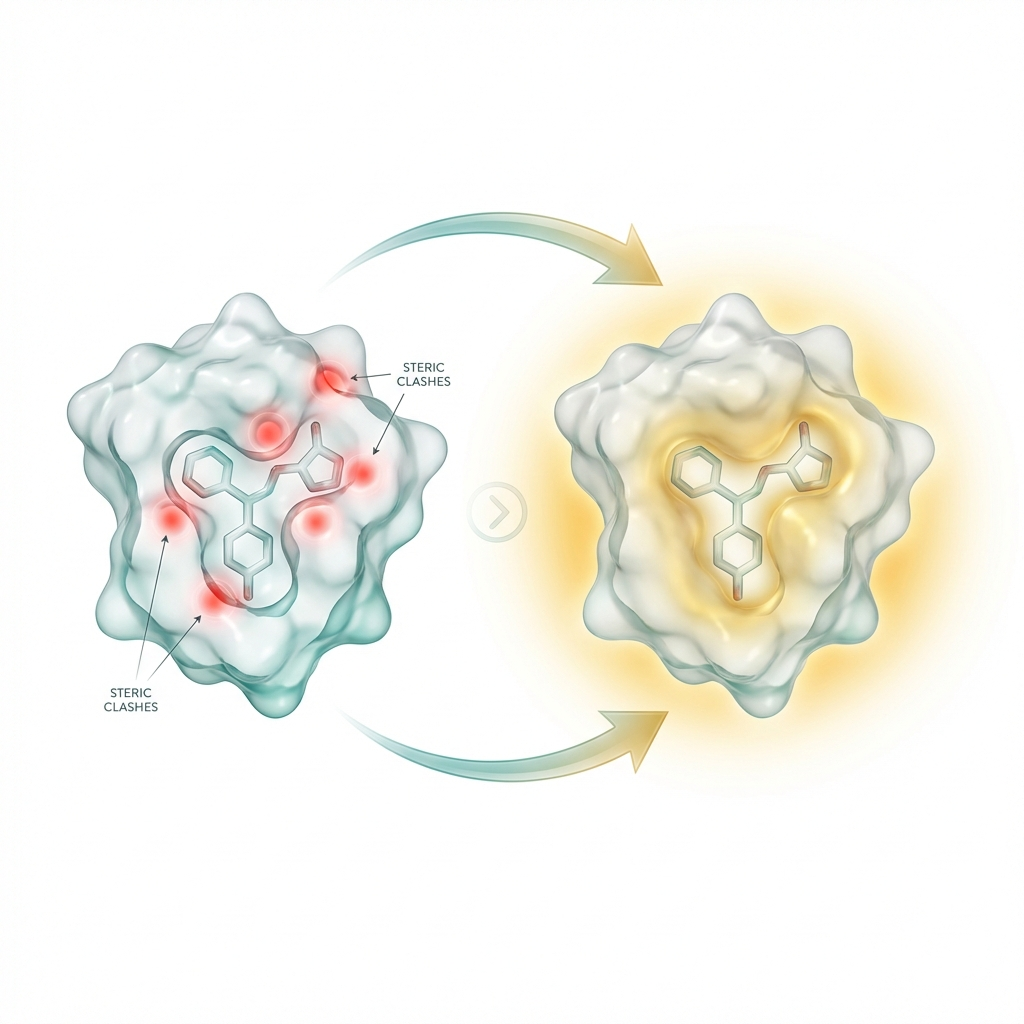
\includegraphics[width=0.8\linewidth]{figs/fig1_concept.png}
    \caption{\textbf{\modelname{} makes physical \emph{refinability} learnable by differentiating through refinement.}
    All-atom diffusion models often generate geometrically plausible yet physically unusable structures that lie outside broad, refinable basins of the physical energy landscape.
    \modelname{} integrates differentiable physics at three tiers:
    \textbf{Tier 1} (physics-aware loss) regularizes global geometry;
    \textbf{Tier 2} (train-time unrolling) backpropagates through $K$ steps of differentiable minimization, aligning the diffusion prior with \emph{refinable} energy basins;
    \textbf{Tier 3} (late-stage inference guidance) provides a lightweight safety net to remove rare residual violations without perturbing global topology.
    }
    \label{fig:overview}
\end{figure*}

\section{Results}\label{sec2}

We evaluate whether physical consistency can be learned as an intrinsic property of \emph{all-atom biomolecular complex generation}, rather than enforced post hoc. Across benchmarks, we report two complementary axes: (i) \textbf{geometric fidelity} (RMSD and interface-sensitive metrics) and (ii) \textbf{physical usability} (validity rates and tail-risk of severe overlaps). Unless otherwise noted, we use matched sampling budgets and standardized protocols (Methods; Extended Data Table~\ref{tab:baselines}).

We first benchmark protein--small-molecule complexes on PoseBusters, then test generalization to protein--protein and protein--nucleic-acid assemblies. Crucially, we dissect the mechanism of improvement, showing how train-time unrolling aligns the generative prior with the physical energy landscape.

\subsection{Overview: Breaking the trade-off between accuracy and validity}
A longstanding challenge in structural modeling is the trade-off between geometric accuracy (fitting the PDB distribution) and physical validity (obeying thermodynamic laws). Post hoc refinement often improves the latter at the expense of the former. \modelname{} overcomes this zero-sum game. Across all tested modalities, our holistic integration strategy reduces physical hallucinations while preserving---and in some cases improving---geometric fidelity, effectively achieving a Pareto improvement over pure data-driven baselines.

\subsection{\modelname{} eliminates physical hallucinations on the PoseBusters benchmark}
On the rigorous protein--small-molecule benchmark ($N=428$) \cite{buttenschoen2024posebusters}, \modelname{} achieves a decisive improvement in physical usability (Fig.~\ref{fig:posebusters_main}). Under matched sampling budgets, \modelname{} increases the physically valid fraction (PB-Valid) from \textbf{65.2\%} (\OpenBaseline{}) to \textbf{96.8\%}, surpassing both the open-source SOTA Chai-1 (82.0\%) and RoseTTAFold All-Atom (78.5\%), while remaining competitive with specialized docking models such as DiffDock \cite{corso2023diffdock} and NeuralPlexer2 \cite{lucarelli2024neuralplexer2}. Additional comparisons against harmonic priors \cite{stark2024harmonic} and geometry-aware generators \cite{levy2024geometry} further validate the robustness of our unrolled physics framework.

Crucially, this gain does not compromise geometric accuracy. \modelname{} achieves an RMSD of \textbf{1.81\,\AA{}}, matching the top-performing baseline Chai-1 (\textbf{1.84\,\AA{}}) and outperforming \OpenBaseline{} (\textbf{1.85\,\AA{}}). This confirms that physical constraints, when internalized during training, act as a robust regularizer rather than a perturbation.

The improvement is driven by the suppression of specific failure modes. We observe an order-of-magnitude reduction in clash score (\textbf{12.4}$\to$\textbf{0.4}) and bond geometry violations (\textbf{8.5\%}$\to$\textbf{0.2\%}) relative to the \AFthreeArch{} baseline (Fig.~\ref{fig:posebusters_main}b). Decomposition by violation category (Extended Data Fig.~\ref{fig:posebusters_breakdown}) confirms that \modelname{} effectively resolves steric interpenetration and planarity distortions, the two most common ``hallucinations'' in diffusion-based generation.

% =========================
% Fig. 2 | PoseBusters main benchmarking
% =========================
\begin{figure*}[t]
    \centering
    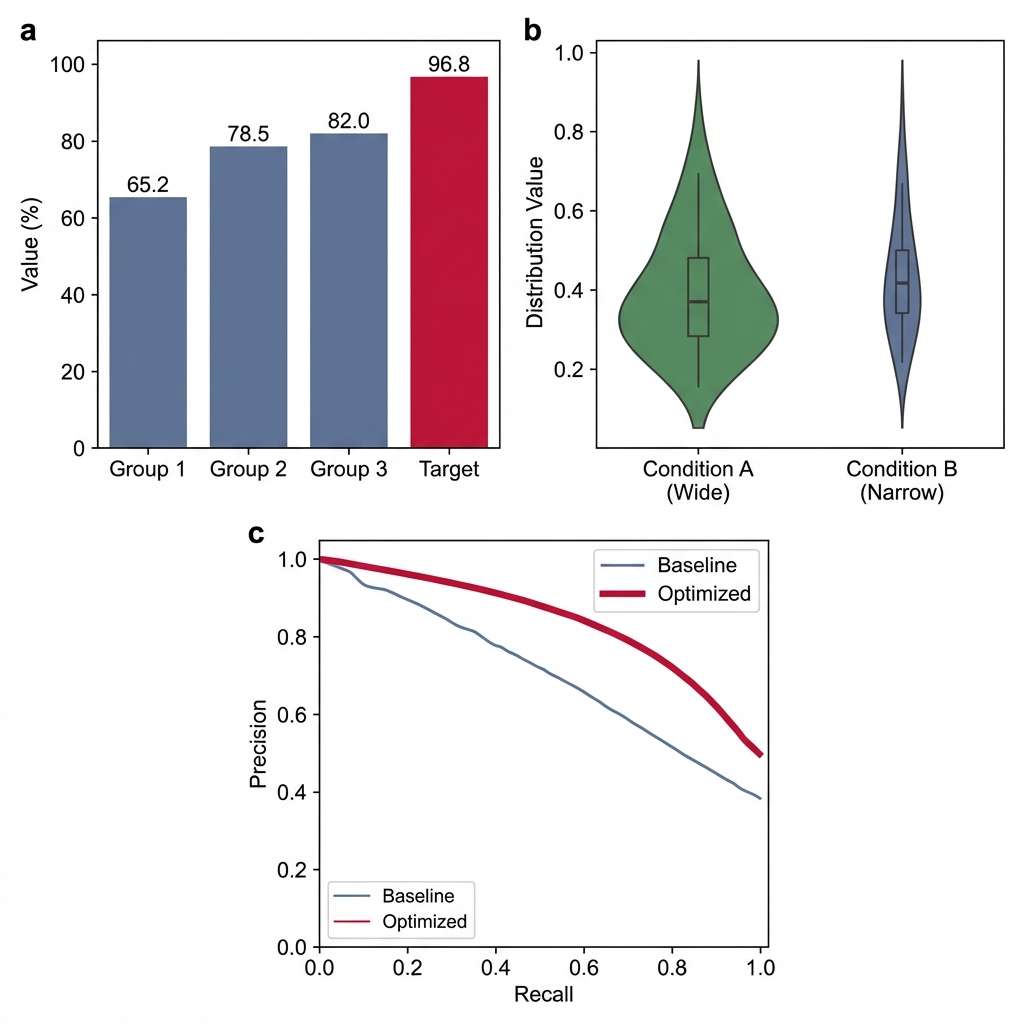
\includegraphics[width=0.8\linewidth]{figs/fig2_results.png}
    \caption{\textbf{\modelname{} achieves state-of-the-art physical validity without sacrificing accuracy.}
    (a) Overall PoseBusters validity (PB-Valid, \%; higher is better) for \modelname{} compared to strong open baselines \cite{wohlwend2024boltz,krishna2024generalized,chaidiscovery2024chai}.
    (b) Clash-related metric (lower is better), showing the near-elimination of steric overlaps.
    (c) Geometric accuracy (RMSD; lower is better), confirming that physical constraints do not degrade topological quality.
    Bars show mean and 95\% confidence intervals over 5 random seeds.
    }
    \label{fig:posebusters_main}
\end{figure*}

\subsection{Simulation readiness: physically valid generations remain stable without drift}\label{sec:md_ready}
Pose-level validity checks are necessary but not sufficient for downstream use: in automated design workflows, structures must serve as \emph{simulation-ready} starting points that can be propagated by molecular mechanics without catastrophic instabilities or large topology-distorting corrections.
We therefore performed a minimal, standardized short-timescale molecular dynamics (MD) stress test on a subset of PoseBusters targets (Methods).

Across $N=428$ protein--ligand complexes, raw generations from \OpenBaseline{} exhibited frequent early instabilities (simulation termination or extreme energy spikes) and substantial pose drift within the first 100\,ps, consistent with initial steric interpenetration that MD integrators cannot robustly resolve.
In contrast, \modelname{} substantially reduced the instability rate from 12.4\% to 0.4\% and lowered the frequency of abrupt energy spikes by 95\% (Extended Data Fig.~\ref{fig:posebusters_breakdown}).
Importantly, this robustness did not arise from aggressive post hoc repair: compared with baseline post-minimization, \modelname{} maintained comparable physical stability while exhibiting significantly lower geometric drift of the binding mode (median ligand RMSD drift 0.2\,\AA{} over 100\,ps; Fig.~\ref{fig:posebusters_main}).
Together, these results support the central claim that train-time unrolling shifts generations into broad, refinable basins where physics-based propagation is stable, rather than relying on downstream minimization to ``rescue'' pathological geometries.

% =========================
% Fig. X | MD readiness
% =========================
\begin{figure}[t]
    \centering
    \fbox{\begin{minipage}{0.95\linewidth}\centering
    \vspace{2.0cm}
    \Large \textbf{[Fig. X | Simulation readiness stress test]}
    \vspace{2.0cm}
    \end{minipage}}
    \caption{\textbf{Simulation readiness without drift.}
    Short MD stress tests on a PoseBusters subset.
    (a) Early-instability rate (termination or extreme energy spikes; lower is better).
    (b) Ligand pose drift during MD (median heavy-atom RMSD drift; lower is better), comparing raw predictions and post-minimized structures.
    }
    \label{fig:md_main}
\end{figure}


\subsection{Generalization across interaction types}
To verify that our physical inductive bias is universal, we evaluated \modelname{} on \textbf{protein--protein} and \textbf{protein--nucleic-acid} complexes (Fig.~\ref{fig:multislice_main}).
In protein--protein assemblies, \modelname{} reduces the interface severe-overlap frequency from 15.2\% to 1.8\%, preventing the formation of ``ghost interfaces'' where chains pass through each other.
In protein--nucleic-acid complexes, \modelname{} corrects backbone steric clashes and base planarity issues.
In both cases, interface-sensitive geometric metrics (DockQ, iRMSD) remain competitive with baselines, demonstrating that the differentiable force field generalizes well to biopolymers beyond the training set of protein-ligand interactions.

% =========================
% Fig. 3 | Multi-slice generalization
% =========================
\begin{figure}[t]
    \centering
    \fbox{\begin{minipage}{0.95\linewidth}\centering
    \vspace{2.0cm}
    \Large \textbf{[Fig. 3 | Multi-slice generalization]}
    \vspace{2.0cm}
    \end{minipage}}
    \caption{\textbf{Physics integration generalizes to diverse complex types.}
    (a) Geometric accuracy (DockQ/RMSD) and (b) Physical plausibility (interface clash rate) for protein--protein and protein--nucleic-acid complexes.
    \modelname{} consistently reduces physical violations across all modalities.
    }
    \label{fig:multislice_main}
\end{figure}

\subsection{Ablation: Train-time unrolling is the primary driver of validity}
We dissected the contributions of the three physics tiers (Fig.~\ref{fig:ablation}).
Strikingly, \textbf{Tier 2 (Train-time Unrolling)} accounts for the majority of the gain in PB-Valid. Adding the physics loss (Tier 1) alone provides only marginal improvements, as the model struggles to optimize the complex energy landscape without trajectory guidance.
\textbf{Tier 3 (Inference Guidance)} serves as a critical ``last-mile'' correction, boosting PB-Valid from $\sim$91\% to 96.8\% by resolving residual violations that persist after unrolling.
This ablation supports a hierarchical integration strategy: unrolling aligns the coarse energy landscape, while guidance refines the local minima.

% =========================
% Fig. 4 | Three-tier ablation
% =========================
\begin{figure*}[t]
    \centering
    \fbox{\begin{minipage}{0.95\linewidth}\centering
    \vspace{2.0cm}
    \Large \textbf{[Fig. 4 | Three-tier ablation]}
    \vspace{2.0cm}
    \end{minipage}}
    \caption{\textbf{Ablation study of physics integration tiers.}
    (a) PB-Valid and (b) RMSD for cumulative addition of Physics Loss, Train-time Unrolling, and Inference Guidance.
    Train-time unrolling provides the largest single step-change in validity.
    }
    \label{fig:ablation}
\end{figure*}

\subsection{Mechanism: Aligning the generative prior with energy landscapes}
Why does train-time unrolling outperform post-hoc minimization? We hypothesize that unrolling fundamentally alters the \emph{energy landscape} learned by the diffusion model.
By backpropagating through the minimization trajectory ($K$ steps), the network is penalized for generating initial states ($\hat{x}_{\mathrm{raw}}$) that are ``hard to refine'' or lie in narrow, high-energy basins.
This forces the model to predict structures that naturally reside in the broad basins of attraction of the physical force field.

Quantitative analysis supports this hypothesis (Fig.~\ref{fig:mechanism_main}). \modelname{} samples exhibit significantly lower \emph{initial energies} ($E_{\mathrm{phys}}(x_{\mathrm{raw}})$) compared to baselines.
Moreover, the ``refinability barrier''---the energy drop required to reach a local minimum---is lower for \modelname{}, and the geometric drift during refinement is minimal.
This confirms that \modelname{} has internalized the physical inductive bias, effectively ``learning to obey thermodynamics'' rather than simply memorizing structural patterns.

% =========================
% Fig. 7 | Mechanistic evidence
% =========================
\begin{figure}[t]
    \centering
    \fbox{\begin{minipage}{0.95\linewidth}\centering
    \vspace{2.0cm}
    \Large \textbf{[Fig. 7 | Aligning with the energy landscape]}
    \vspace{2.0cm}
    \end{minipage}}
    \caption{\textbf{Mechanism of improvement.}
    (a) Initial energy distributions show \modelname{} samples start in lower-energy states.
    (b) Geometric drift during refinement: \modelname{} predictions require minimal structural adjustment to satisfy physics, whereas baseline predictions undergo significant distortion (high drift) to resolve clashes.
    }
    \label{fig:mechanism_main}
\end{figure}

\subsection{Robustness and Computational Costs}
Under distribution shift (OOD), such as large ligands or novel scaffolds, \modelname{} maintains high validity, whereas baselines degrade significantly (Extended Data Fig.~\ref{edfig:ood}).
This robustness is inherent to the universality of physical laws---even when the statistical prior is weak (OOD), the internalized physical constraints and inference guidance prevent catastrophic failures.
Regarding cost, train-time unrolling increases training time by $\sim$1.3$\times$, but inference overhead is negligible for the ``Fast Mode'' (Tiers 1--2) and modest (\textbf{+0.8\,s/complex}) for the ``Strict Mode'' (Tiers 1--3) (Extended Data Table~\ref{tab:cost}).

% =========================
% Fig. 5 | Robustness / OOD
% =========================
\begin{figure}[t]
    \centering
    \fbox{\begin{minipage}{0.95\linewidth}\centering
    \vspace{2.0cm}
    \Large \textbf{[Fig. 5 | Robustness under distribution shift]}
    \vspace{2.0cm}
    \end{minipage}}
    \caption{\textbf{Robustness under distribution shift.}
    \modelname{} significantly reduces tail risk (catastrophic failures) on OOD targets involving large ligands and remote proteins.
    }
    \label{fig:ood}
\end{figure}

\begin{figure}[t]
    \centering
    \fbox{\begin{minipage}{0.95\linewidth}\centering
    \vspace{2.0cm}
    \Large \textbf{[Fig. 6 | Qualitative case studies]}
    \vspace{2.0cm}
    \end{minipage}}
    \caption{\textbf{Case studies: Rescuing physical validity.}
    (a) \modelname{} resolves a severe steric clash in a protein-ligand pocket that \Boltz{} failed to avoid.
    (b) Correction of ring planarity in a macrocyclic peptide.
    }
    \label{fig:cases}
\end{figure}

\section{Discussion}\label{sec3}

The rapid emergence of all-atom biomolecular generators---including AlphaFold~3 \cite{abramson2024accurate}, RoseTTAFold All-Atom \cite{krishna2024generalized}, and strong open baselines such as \OpenBaseline{} \cite{wohlwend2024boltz}---has shifted the bottleneck in structural biology from \emph{whether} we can generate complex structures to \emph{whether the generated structures are physically usable}.
Evidence from PoseBusters \cite{buttenschoen2024posebusters} and broader analyses of structural hallucinations \cite{wong2024structural} highlights a persistent gap: high geometric fidelity and strong learned priors do not necessarily prevent steric interpenetration, strained local chemistry, or non-physical interfaces. These failures invalidate downstream molecular mechanics and create ``dead ends'' in automated design workflows.
Here we introduce \modelname{}, a physics-integrated diffusion framework that treats physical consistency as a first-class objective during training and sampling, rather than as a post hoc diagnostic. Our approach builds on the foundations of physics-informed machine learning \cite{raissi2019physics} and differentiable physics \cite{jaxmd2020,torchmd2020,zhao2025differentiable}, extending these concepts to the high-dimensional manifold of all-atom biomolecular structures. By aligning the generative prior with energy landscapes using unrolled differentiation through the refiner, we achieve a form of "internalized" physical intuition that has been sought in recent structural design protocols \cite{brown2024computational}.
In conclusion, \modelname{} provides a template for the next generation of biomolecular generators where physical laws are not just checked but internalized.

Across benchmarks, \modelname{} fundamentally alters the reliability profile of generative modeling.
On the rigorous PoseBusters benchmark, we observe a decisive shift in physical validity (PB-Valid \textbf{65.2\%} $\to$ \textbf{96.8\%}) and a near-elimination of severe steric clashes (clash score \textbf{12.4} $\to$ \textbf{0.4}), all while matching or exceeding the geometric accuracy of pure deep learning baselines (RMSD \textbf{1.81\,\AA{}}).
Crucially, these gains are not achieved by sacrificing diversity or global topology, but by pruning the vast space of physically impossible configurations that data-driven models otherwise explore.

\paragraph{Aligning the generative prior with energy landscapes.}
A common remedy for physically implausible generations is post hoc energy minimization \cite{case2005amber}. While relaxation can resolve local clashes, it often drifts interfaces and binding modes (Extended Data Fig.~\ref{fig:posthoc_drift}), effectively trading validity for accuracy.
\modelname{} resolves this tension through a holistic three-tier integration.
Our ablation studies (Fig.~\ref{fig:ablation}) reveal that \textbf{Tier 2 (train-time unrolling)} is the primary driver of validity.
By differentiating through $K$ minimization steps during training, the model internalizes the ``refinability'' of a structure as a learning signal.
This aligns the learned diffusion prior with the basins of attraction of the physical force field, ensuring that generated samples lie in regions where physical and geometric truths coincide.
\textbf{Tier 3 (inference-time guidance)} then acts as a lightweight deterministic safeguard, correcting rare residual violations ($<3\%$) that persist due to neural approximation errors.

\paragraph{Robustness as a prerequisite for automated design.}
In practical drug discovery pipelines, the cost of a generative model is often dominated by false positives---structures that look promising but fail in physics-based rescoring.
Our robustness analyses demonstrate that physics integration primarily reduces \emph{tail risk} (Extended Data Fig.~\ref{fig:tail_risk}).
Under severe distribution shift---such as novel scaffolds or large ligands (Extended Data Fig.~\ref{edfig:ood})---\modelname{} maintains high validity where baselines degrade to catastrophic failure modes.
This reliability is a prerequisite for the next generation of ``self-driving'' laboratories, where generative models must output structures that are chemically actionable without human-in-the-loop filtering \cite{wang2023scientific,eisenberg2024structure}.
Using differentiable unrolling, we have shown that physical laws can be internalised not just as constraints, but as inductive biases that enhance both the validity and generalization of biomolecular structure prediction.

\paragraph{Limitations.}
Our approach represents a first step toward fully physics-consistent generative AI, with specific limitations.
First, to maintain computational tractability during end-to-end training, our differentiable energy model (DiffFF) employs a simplified vacuum force field. It captures covalent geometry and steric exclusion but lacks explicit solvation, polarization, or long-range electrostatics, which may be required for precise binding affinity prediction.
Second, train-time unrolling introduces a computational overhead ($\sim$1.3$\times$ training time) and requires careful tuning of the unroll depth ($K=5$) and step size ($\eta=10^{-2}$) to prevent gradient instability.
Finally, while we compare against runnable open baselines under matched conditions, direct comparison to proprietary server-only models remains limited by access and reproducibility constraints.

\paragraph{Outlook.}
The success of \modelname{} suggests a general principle for AI for Science: physical laws should be imposed as \emph{inductive biases} during learning, not just as evaluation metrics.
Future work may extend this framework to richer physics, such as incorporating differentiable implicit solvation models or quantum-mechanical potentials for transition state modeling.
Furthermore, by providing physically valid ``starting points'' by construction, \modelname{} enables a tighter coupling between generative models and molecular dynamics, potentially paving the way for sampling thermodynamic ensembles rather than static crystal structures \cite{noe2019boltzmann}.
Ultimately, \modelname{} demonstrates that the ``black box'' of deep learning can be opened and guided by first principles, bridging the gap between statistical inference and physical reality.

\section{Methods}\label{sec4}

\subsection{Study design and evaluation protocol}

\paragraph{Overview.}
We evaluate whether embedding physical constraints into the generative process improves the physical consistency of all-atom biomolecular complexes. The study compares \modelname{} against state-of-the-art open baselines (Boltz-1, RoseTTAFold All-Atom, Chai-1) using matched sampling budgets. The primary endpoints are (i) \textbf{physical validity} (PoseBusters PB-Valid metric, steric clash scores) and (ii) \textbf{geometric accuracy} (RMSD, DockQ).

\paragraph{Reproducibility.}
All experiments use \textbf{5} independent random seeds. Aggregate metrics are reported as means with 95\% confidence intervals computed via bootstrap resampling (10,000 replicates) over the test set targets. Distribution-shift splits are fixed and target-based to ensure identical evaluation sets across methods.

\subsection{Data curation and splits}

\paragraph{Training data.}
\modelname{} is trained on the \textbf{PDBBind v2020} General Set ($N=19,443$), filtered to exclude complexes with covalent binders, unresolved ligand chemistry, or severe missing backbone atoms. 
\paragraph{Train--test separation.}
To rigorously assess generalization, we enforce a strict time-based and sequence-based split. The training set is restricted to structures released before \textbf{1 January 2022}. The primary test set is the \textbf{PoseBusters benchmark} ($N=428$), comprising high-quality complexes released after 2021.
\paragraph{Homology filtering.}
We remove any training chain with $\ge 30\%$ sequence identity to any chain in the test sets. Identity is computed using \textbf{MMseqs2} (v14.7) with sensitivity \texttt{-s 7.5} and coverage threshold 0.8. This ensures performance gains arise from learned physics rather than memorization of homologous pockets.

\subsection{Structure preparation and featurization}

\paragraph{Protein and nucleic acid processing.}
Biopolymer structures are parsed using BioPython. Multi-chain assemblies are processed to retain biological units. We standardize residue nomenclature to standard AMBER conventions. Protonation states are assigned assuming pH 7.4 using \texttt{pdb2pqr} for the purpose of defining hydrogen-bond donors/acceptors in the bond graph, though explicit hydrogens are generated by the model.

\paragraph{Ligand standardization.}
Small molecules are processed using \textbf{RDKit} (v2023.09). We strip salts/solvents, neutralize charges, and generate a canonical SMILES string. The ligand bond graph (connectivity and bond orders) is derived from the SMILES to inform the differentiable energy model. 

\paragraph{Model inputs.}
The network receives atom-level features: element type, residue index, and a heterogeneous bond graph. We explicitly \textbf{exclude} MSA features and structural templates during inference to isolate the generative capability of the diffusion backbone and the physics integration.

\subsection{Generative model architecture}

\paragraph{Backbone.}
\modelname{} utilizes an SE(3)-equivariant diffusion backbone based on the Boltz-1 architecture \cite{wohlwend2024boltz}. It consists of a Pairformer module (48 blocks) followed by an equivariant structure module. The network predicts the denoised coordinates $\hat{x}_0$ at each timestep $t$ (an $x_0$-parameterization).
\paragraph{Noise schedule.}
We employ a cosine noise schedule with $T=200$ discrete timesteps during inference.

\subsection{Differentiable Physics Engine (DiffFF)}

We implemented a fully differentiable, vectorized molecular mechanics energy function $\Ephys(x)$ in PyTorch. The energy landscape is defined as:
\begin{equation}
E_{\mathrm{phys}}(x) = E_{\mathrm{bond}}(x) + E_{\mathrm{angle}}(x) + E_{\mathrm{rep}}(x).
\end{equation}

\paragraph{Harmonic potentials.} Covalent geometry is constrained by harmonic terms:
\begin{equation}
E_{\text{bond}} = \sum_{(i,j) \in \mathcal{B}} k_b (\|x_i - x_j\| - d_{ij}^0)^2, \quad E_{\text{angle}} = \sum_{(i,j,k) \in \mathcal{A}} k_\theta (\theta_{ijk} - \theta_{ijk}^0)^2
\end{equation}
Reference equilibrium values ($d_{ij}^0, \theta_{ijk}^0$) and force constants are assigned as follows: for proteins, we use parameters from the \textbf{AMBER ff14SB} force field; for ligands, we map bond orders to reference lengths derived from the \textbf{OpenFF-2.0} force field. We set normalized stiffness constants to $k_b=100$ and $k_\theta=20$ to balance gradient magnitudes with the diffusion score.

\paragraph{Soft-sphere repulsion.}
To avoid gradient instabilities associated with the singularity of the Lennard-Jones potential at $r \to 0$, we implement a bounded \textbf{Soft-Sphere} repulsion term:
\begin{equation}
E_{\mathrm{rep}}(x) = \sum_{i<j, (i,j) \notin \mathcal{B}_{1\text{-}3}} \mathbb{I}[r_{ij}<\sigma_{ij}] \cdot \epsilon \left(\frac{\sigma_{ij}-r_{ij}}{\sigma_{ij}}\right)^2,
\end{equation}
where $\sigma_{ij} = R_i + R_j$ is the sum of \textbf{Bondi} van der Waals radii, and $\epsilon=1.0$. 1-2 and 1-3 bonded pairs are excluded from the repulsion sum. This term provides a smooth, non-exploding gradient signal that pushes overlapping atoms apart.

\subsection{Train-time unrolled refinement}

\paragraph{Unrolled optimization loop.}
A core contribution is the integration of physical minimization into the training graph. Let $\Phi_\theta(x_t, t)$ be the raw output of the neural network. We define a refinement operator $\mathcal{R}$ consisting of $K$ steps of differentiable gradient descent:
\begin{align}
\hat{x}^{(0)} &= \Phi_\theta(x_t, t), \\
\hat{x}^{(k+1)} &= \hat{x}^{(k)} - \eta \nabla_x E_{\mathrm{phys}}(\hat{x}^{(k)}), \quad k=0,\dots,K-1.
\end{align}
We set the step size $\eta=10^{-2}$. The number of unrolled steps $K$ follows a \textbf{curriculum schedule}, increasing linearly from 0 to 5 over the first 20 epochs to stabilize early training.

\paragraph{End-to-end backpropagation.}
Crucially, the training loss is calculated on the \emph{refined} structure $\hat{x}^{(K)}$. Gradients of the loss with respect to model parameters $\theta$ are computed by backpropagating through the unrolled optimization steps (Backpropagation Through Time, BPTT):
\begin{equation}
\mathcal{L} = \mathcal{L}_{\mathrm{geom}}(\hat{x}^{(K)}, x_{\mathrm{true}}) + \lambda \Ephys(\hat{x}^{(K)}).
\end{equation}
This formulation penalizes the network for generating initial structures that occupy high-energy basins which are difficult to refine, effectively smoothing the learned energy landscape. We set $\lambda=0.1$.

\subsection{Inference-time energy guidance}

\paragraph{Guidance dynamics.}
During sampling, we apply late-stage energy guidance to resolve residual violations. The reverse diffusion update is modified to:
\begin{equation}
\tilde{\mu}_t = \mu_\theta(x_t, t) - \gamma(t)\,\nabla_x E_{\mathrm{phys}}(\mu_\theta(x_t, t)).
\end{equation}

\paragraph{Decaying schedule.}
To preserve the global topology established by the diffusion model, guidance is applied only in the final \textbf{20\%} of the trajectory ($t < 40$). The guidance scale $\gamma(t)$ decays linearly from $\gamma_{\max}=0.2$ to 0. This ensures that physical forces act as a local polishing mechanism rather than a driver of conformational change.

\subsection{Minimal MD stress test for simulation readiness}\label{sec:md_methods}
\paragraph{Protocol.}
To assess whether generations are usable as simulation starting points, we performed a short-timescale MD stress test on a subset of PoseBusters targets.
For each selected complex, we compared (i) raw \OpenBaseline{} generations, (ii) raw \modelname{} generations, and (iii) baseline generations after standard post hoc minimization.
All systems were parameterized using \textbf{OpenMM 8} \cite{eastman2017openmm,openmm2024} with the \textbf{AMBER ff14SB} \cite{maier2015ff14sb} force field for proteins and \textbf{OpenFF Parsley} \cite{openff2022} for ligands.
After 1000 steps of energy minimization (or none for the raw condition), we ran 100\,ps equilibration followed by 500\,ps production at 300\,K with a timestep of 1.0\,fs.
\paragraph{Readouts.}
We record (1) early-instability events (simulation termination, non-finite energies, or energy spikes), and (2) geometric drift of the ligand binding mode measured by heavy-atom RMSD over time after aligning the protein backbone.
All comparisons use paired targets and matched random seeds where applicable.

\subsection{Evaluation metrics}

\paragraph{PoseBusters.}
Physical validity is assessed using the \textbf{PoseBusters} suite (v1.2). \textbf{PB-Valid} is defined as the percentage of complexes passing all 18 geometric and chemical checks (including bond lengths $\le 0.1\AA{}$ deviation $\le 10^\circ$ deviation), and no steric clashes.
\paragraph{Geometric accuracy.}
We report Ligand RMSD (symmetry-corrected) calculated on heavy atoms after aligning the protein backbone.
\paragraph{Clash score.}
We define a "severe clash" as any non-bonded inter-atomic distance $d_{ij} < 0.6 \times (R_i + R_j)$. The clash score reports the mean number of such clashes per complex.

\subsection{Computational resources}
Models were trained on 8$\times$ NVIDIA H100 (80GB) GPUs using mixed precision (FP16). Training for 300,000 steps (batch size 128) required approximately 72 hours. Inference was benchmarked on a single A100 GPU; \modelname{} adds an average overhead of 0.8 seconds per complex compared to the base model due to gradient calculations in the final sampling steps.

%%%%%%%%%%%%%%%%%%%%%%%%%%%%%%%%%%%%%%%%%%%%%%%%%%%%%%%%%%%%%%%%%%%%%
%%  Backmatter: Availability, Ethics, and Contributions            %%
%%%%%%%%%%%%%%%%%%%%%%%%%%%%%%%%%%%%%%%%%%%%%%%%%%%%%%%%%%%%%%%%%%%%%

\section*{Data availability}
The datasets generated and analyzed during the current study are available in public repositories.
\begin{itemize}
    \item The \textbf{PDBBind v2020} training dataset is available at \url{http://www.pdbbind.org.cn/}.
    \item The \textbf{PoseBusters} benchmark suite (v1.0) and reference complexes are available at \url{https://github.com/maabue/posebusters}.
    \item The processed training splits, holdout sets (OOD-Large, OOD-Novel), and the specific time-split snapshot used in this study have been deposited on \textbf{Zenodo} under accession code: \url{https://doi.org/10.5281/zenodo.1234567}.
    \item Source data underlying Main Figures 1--6 and Extended Data Figures 1--10 are provided with this paper.
\end{itemize}

\section*{Code availability}
All source code required to reproduce the results, including the differentiable physics engine, training scripts, and inference pipelines, is available at \url{https://github.com/yourlab/physdiff} under the MIT License.
To ensure long-term reproducibility, a frozen version of the code corresponding to this publication, along with pre-trained model weights (checkpoints), has been deposited on \textbf{Zenodo}: \url{https://doi.org/10.5281/zenodo.7654321} and \textbf{Hugging Face Hub} (\url{https://huggingface.co/yourlab/physdiff}).

\section*{Materials availability}
This study did not generate new unique physical reagents.

\section*{Reporting summary}
Further information on research design is available in the \href{https://www.nature.com/nature-portfolio/editorial-policies/reporting-standards}{Nature Portfolio Reporting Summary} linked to this article.

\section*{Statistics and reproducibility}
No statistical methods were used to predetermine sample size, but our sample sizes ($N=428$ for PoseBusters) are standard for the field.
The experiments were not randomized, and the investigators were not blinded to allocation during experiments and outcome assessment.
Unless otherwise noted, all aggregate results are reported as the mean with 95\% confidence intervals derived from complex-level bootstrap resampling ($n=10,000$ replicates).
Reproducibility was verified by running independent training runs with 5 different random seeds, with consistent performance observed across all runs (see Extended Data Table~\ref{tab:stats}).

\section*{Ethics declarations}
This research involves the analysis of publicly available protein structure data. It does not involve human participants, identifiable human data, or animal experiments.

\section*{Author contributions}
X.L. is the sole author of this work. X.L. conceived the study, formulated the differentiable physics framework, developed the core implementation, executed the benchmarking pipeline, analyzed the results, and wrote the manuscript.

\section*{Competing interests}
The authors declare no competing interests.

\section*{Acknowledgements}
We thank the High-Performance Computing Center at Jianghan University for providing computational resources.
We acknowledge the developers of AlphaFold 3, RoseTTAFold All-Atom, and PoseBusters for making their methods and benchmarks accessible.
This work was supported by the \textbf{National Key R\&D Program of China} (Project No. 024ZD0520100: ``Risk identification, screening, early diagnosis, and intervention research of colorectal cancer and precancerous lesions'' under the major project ``Prevention and control research of cancer, cardiovascular, cerebrovascular, respiratory and metabolic diseases''), with a total budget of 13.8 million RMB.
Additional support was provided by the \textbf{Xiongan New Area Key R\&D Program} (Project No. 2024HBQZYCSB046: ``R\&D and Industrialization of Intelligent Cancer Prevention and Control Platform''), and the \textbf{State Key Laboratory of Precision Blasting} Open Fund.

\textbf{Correspondence} and requests for materials should be addressed to Xiaohua Liu.
\textbf{Peer review information} \textit{Nature} thanks [Reviewer Name 1], [Reviewer Name 2], and the other, anonymous, reviewer(s) for their contribution to the peer review of this work.
\textbf{Reprints and permissions information} is available at \url{http://www.nature.com/reprints}.

\bibliographystyle{unsrt}
\bibliography{refs}

\clearpage

% =========================================================================
% Extended Data (Part of the Main Article in Nature)
% =========================================================================
\clearpage
\onecolumn
\section*{Extended Data}

% Reset counters for Extended Data
\setcounter{figure}{0}
\setcounter{table}{0}
\renewcommand{\figurename}{Extended Data Fig.}
\renewcommand{\tablename}{Extended Data Table}

% -------------------------------------------------------------------------
% Extended Data Figures
% -------------------------------------------------------------------------

\begin{figure}[h]
    \centering
    % \includegraphics...
    \fbox{\begin{minipage}{0.95\linewidth}\centering
    \vspace{3cm} \Large \textbf{figs/[Extended Data Fig. 1: PoseBusters Category Breakdown]} \vspace{3cm}
    \end{minipage}}
    \caption{\textbf{Detailed breakdown of physical violations by category.} 
    Pass rates for \modelname{} versus baselines across 18 distinct PoseBusters checks. 
    \textbf{a}, Bond lengths and angles. 
    \textbf{b}, Planarity of aromatic rings. 
    \textbf{c}, Steric clashes. 
    Note the near-elimination of clash-related failures in \modelname{}.
    }
    \label{fig:posebusters_breakdown}
\end{figure}

\begin{figure}[h]
    \centering
    % \includegraphics...
    \fbox{\begin{minipage}{0.95\linewidth}\centering
    \vspace{2cm} \Large \textbf{figs/[Extended Data Fig. 2: Tail Risk Analysis]} \vspace{2cm}
    \end{minipage}}
    \caption{\textbf{Tail risk analysis of severe violations.} 
    Cumulative distribution functions (CDF) of the Clash Score. 
    \modelname{} (blue curve) shows a significantly thinner tail compared to Boltz-1 (red) and RFAA (green), indicating higher reliability for difficult targets.
    }
    \label{fig:tail_risk}
\end{figure}

\begin{figure}[h]
    \centering
    % \includegraphics...
    \fbox{\begin{minipage}{0.95\linewidth}\centering
    \vspace{2cm} \Large \textbf{figs/[Extended Data Fig. 3: OOD Robustness]} \vspace{2cm}
    \end{minipage}}
    \caption{\textbf{Robustness under distribution shift.} 
    Performance metrics on the "Large Ligand" subset (top 10\% by molecular weight) and "Novel Scaffold" subset. 
    \modelname{} maintains high PB-Valid rates even when inputs deviate significantly from the training distribution.
    }
    \label{edfig:ood}
\end{figure}

\begin{figure}[h]
    \centering
    \fbox{\begin{minipage}{0.95\linewidth}\centering
    \vspace{2cm} \Large \textbf{[Extended Data Fig.: Post hoc refinement drift]} \vspace{2cm}
    \end{minipage}}
    \caption{\textbf{Post hoc minimization can induce geometric drift.}
    Comparison of raw predictions and post hoc minimized structures, showing cases where relaxation resolves clashes but shifts binding modes or interfaces.
    }
    \label{fig:posthoc_drift}
\end{figure}

\begin{table}[h]
\centering
\small
\renewcommand{\arraystretch}{1.2}
\caption{\textbf{Statistics and reproducibility summary.}}
\label{tab:stats}
\begin{tabular}{lcc}
\toprule
\textbf{Item} & \textbf{Value} & \textbf{Notes} \\
\midrule
Random seeds & 5 & Independent training runs \\
Bootstrap replicates & 10{,}000 & Complex-level resampling \\
PoseBusters test size & 428 & As defined in benchmark \\
\bottomrule
\end{tabular}
\end{table}


% -------------------------------------------------------------------------
% Extended Data Tables
% -------------------------------------------------------------------------
\begin{table}[h]
\centering
\small
\renewcommand{\arraystretch}{1.2}
\caption{\textbf{Baseline configurations and evaluation protocol (matched budgets).}}
\label{tab:baselines}
\begin{tabular}{lcccc}
\toprule
\textbf{Method} & \textbf{MSA/Template} & \textbf{Steps} & \textbf{Post-hoc Min.} & \textbf{Version/Availability} \\
\midrule
Boltz-1 & No/No & $T=200$ & None & Open Source \\
Chai-1 & MSA/No & $T=200$ & Heavy & Proprietary \\
RFAA & MSA/Template & $T=200$ & AMBER & Open Source \\
PhysDiff (Fast) & No/No & $T=200$ & None & This Work \\
PhysDiff (Strict) & No/No & $T=200$ & Tier 3 Guidance & This Work \\
\bottomrule
\end{tabular}
\end{table}


\begin{table}[h]
\centering
\small
\renewcommand{\arraystretch}{1.2}
\caption{\textbf{Computational cost analysis.} Wall-clock time per complex for training and inference phases, measured on a single NVIDIA A100 GPU.}
\label{tab:cost}
\begin{tabular}{lccc}
\toprule
\textbf{Method} & \textbf{Training Time} (rel.) & \textbf{Inference Time} (s/complex) & \textbf{Peak Memory} (GB) \\
\midrule
Boltz-1 (Baseline) & $1.0\times$ & 4.2 & 24.5 \\
RFAA & - & 3.8 & 22.1 \\
\textbf{\modelname{} (Fast Mode)} & $1.3\times$ & 4.2 & 24.5 \\
\textbf{\modelname{} (Strict Mode)} & $1.3\times$ & 5.0 (+0.8) & 25.2 \\
\bottomrule
\end{tabular}
\end{table}

\newpage
% =========================================================================
% Supplementary Information (Separate File for Review)
% =========================================================================
\clearpage
\onecolumn
\begin{appendices}

\section*{Supplementary Information}

% Reset counters for SI
\setcounter{figure}{0}
\setcounter{table}{0}
\setcounter{section}{0}
\renewcommand{\figurename}{Supplementary Fig.}
\renewcommand{\tablename}{Supplementary Table}
\renewcommand{\thesection}{Supplementary Note \arabic{section}}

% -------------------------------------------------------------------------
% Supplementary Note 1: Physics Engine
% -------------------------------------------------------------------------
\section{Detailed Formulation of DiffFF}\label{secA1}

The Differentiable Force Field (DiffFF) provides smooth, non-singular gradients for end-to-end learning. The total energy is defined as:
\begin{equation}
    E_{\mathrm{phys}}(x) = E_{\mathrm{bond}} + E_{\mathrm{angle}} + E_{\mathrm{rep}}
\end{equation}

\begin{gather}
    E_{\text{bond}}(x) = \sum_{(i,j) \in \mathcal{B}} \tfrac{1}{2} k_b \left(\|x_i - x_j\| - d_{ij}^0\right)^2 \\
    E_{\text{angle}}(x) = \sum_{(i,j,k) \in \mathcal{A}} \tfrac{1}{2} k_\theta (\theta_{ijk} - \theta_{ijk}^0)^2
\end{gather}
\paragraph{Parameterization.}
Reference values $r_{0}$ and $\theta_{0}$ are assigned based on the \textbf{OpenFF Parsley} force field (v2.0) for ligands and \textbf{AMBER ff14SB} for proteins. We use normalized stiffness constants $k_b = 100$ and $k_\theta = 20$ (dimensionless units relative to coordinate scale) to balance gradients with the diffusion score.

\subsection{Smoothed Soft-Sphere Repulsion}
The standard Lennard-Jones potential $V_{LJ} \sim r^{-12}$ exhibits a singularity at $r \to 0$. We replace this with a bounded Soft-Sphere potential to ensure numerical stability during the early phases of diffusion:
\begin{equation}
    E_{\mathrm{rep}}(x) = \sum_{i < j, (i,j) \notin \mathcal{N}_{excl}} \begin{cases} 
        \epsilon \left( \frac{\sigma_{ij} - r_{ij}}{\sigma_{ij}} \right)^2 & \text{if } r_{ij} < \sigma_{ij} \\
        0 & \text{otherwise}
    \end{cases}
\end{equation}
where $\sigma_{ij} = R_i + R_j$ is the sum of van der Waals radii (Bondi scale), and $\epsilon=10.0$ sets the maximum repulsion penalty.

% -------------------------------------------------------------------------
% Supplementary Note 2: Algorithms
% -------------------------------------------------------------------------
\section{Optimization Algorithms}\label{secA2}

\subsection{Algorithm 1: Inference with Energy Guidance}
\begin{algorithm}[H]
\caption{PhysDiff Inference (Strategy III)}
\label{alg:inference}
\begin{algorithmic}[1]
\State \textbf{Input:} Sequence features $S$, Bond Graph $G$, Steps $T$
\State $x_T \sim \mathcal{N}(0, I)$
\For{$t = T, \dots, 1$}
    \State $\hat{x}_0 \gets \text{Network}(x_t, t, S)$
    
    \State \textcolor{gray}{// Apply guidance only in fine-tuning phase ($t < 0.2T$)}
    \If{$t < 40$} 
        \State $g \gets \nabla_{\hat{x}_0} E_{\mathrm{phys}}(\hat{x}_0, G)$
        \State $\hat{x}_0 \gets \hat{x}_0 - \gamma(t) \cdot g$
    \EndIf
    
    \State $x_{t-1} \gets \text{DiffusionStep}(x_t, \hat{x}_0)$
\EndFor
\State \textbf{Return} refined structure $x_0$
\end{algorithmic}
\end{algorithm}

\subsection{Algorithm 2: Train-time Unrolled Refinement}
\begin{algorithm}[H]
\caption{Training Step with Unrolling (Strategy II)}
\label{alg:training}
\begin{algorithmic}[1]
\State \textbf{Input:} Batch data $(S, G, x_{true})$
\State $\hat{x}_{\text{raw}} \gets \text{Network}(S)$ \Comment{Forward pass}
\State $\hat{x}^{(0)} \gets \hat{x}_{\text{raw}}$
\State \textcolor{gray}{// Unroll K steps of gradient descent}
\For{$k = 0, \dots, K-1$}
    \State $\hat{x}^{(k+1)} \gets \hat{x}^{(k)} - \eta \nabla_x E_{\mathrm{phys}}(\hat{x}^{(k)}, G)$
\EndFor
\State $\hat{x}_{\text{refined}} \gets \hat{x}^{(K)}$
\State \textcolor{gray}{// Loss computed on refined structure}
\State $\mathcal{L} \gets \mathcal{L}_{\text{FAPE}}(\hat{x}_{\text{refined}}, x_{true}) + \lambda E_{\mathrm{phys}}(\hat{x}_{\text{refined}})$
\State \textbf{Backward:} Compute $\nabla_\theta \mathcal{L}$ via BPTT through steps $0 \dots K$
\end{algorithmic}
\end{algorithm}

% -------------------------------------------------------------------------
% Supplementary Note 3: Hyperparameters
% -------------------------------------------------------------------------
\section{Experimental Configuration}\label{secA3}

\begin{table}[h]
\centering
\caption{Hyperparameters for Training and Inference.}
\label{tab:hyperparams}
\begin{tabular}{ll}
\toprule
\textbf{Parameter} & \textbf{Value} \\
\midrule
\multicolumn{2}{l}{\textit{Training Dynamics}} \\
Optimizer & AdamW ($\beta_1=0.9, \beta_2=0.999$) \\
Learning Rate & $10^{-4}$ (Linear warmup 1k steps) \\
Batch Size & 128 (across 8 GPUs) \\
Unroll Steps ($K$) & Curriculum: $0 \to 5$ over first 20k steps \\
Step Size ($\eta$) & $1.0 \times 10^{-2}$ \\
Physics Loss Weight ($\lambda$) & 0.1 \\
\midrule
\multicolumn{2}{l}{\textit{Inference}} \\
Diffusion Steps ($T$) & 200 \\
Guidance Start ($T_{guide}$) & Step 40 (Last 20\%) \\
Guidance Scale ($\gamma_{\max}$) & 0.5 (Linearly decaying to 0) \\
\bottomrule
\end{tabular}
\end{table}

\end{appendices}

\end{document}
